% This work is licensed under the Creative Commons
% Attribution-NonCommercial-ShareAlike 4.0 International License. To view a copy
% of this license, visit http://creativecommons.org/licenses/by-nc-sa/4.0/ or
% send a letter to Creative Commons, PO Box 1866, Mountain View, CA 94042, USA.

\section{Elemente der Linearen Algebra}
Ziel: Bereitstellung einiger Hilfsmittel aus der linearen Algebra.
Literatur:
\begin{enumerate}[label=(\arabic*)]
	\item G. Fischer (1997) \emph{Lineare Algebra} \cite{fischerLinAlg}
	\item M. Koecher (1997) \emph{Lineare Algebra und analytische Geometrie} \cite{koecher2013lineare}
\end{enumerate}

Im gesamten Abschnitt ist
\begin{align*}
	\R^n:=\set{\begin{pmatrix}
		x_1\\
		\vdots\\
		x_n
	\end{pmatrix}
	:x_i\in\R\quad\forall 1\leq i\leq n}\qquad\forall n\in\N
\end{align*}
der gewöhnliche \define{euklidische Raum} versehen mit dem kanonischen Skalarprodukt
\begin{align*}
	\scaProd{x}{y}:=\sum\limits_{i=1}^n x_i\mal y_i\qquad\forall x,y\in\R^n
\end{align*}
und zugehöriger \define{euklidische Norm}
\begin{align*}
	\norm{x}:=\sqrt{\scaProd{x}{x}}
	=\sqrt{\sum\limits_{i=1}^n x_i^2}
	\qquad\forall x\in\R
\end{align*}

\setcounter{satz}{-1}
\begin{definition}\label{def2.0}\
	\begin{enumerate}[label=(\arabic*)]
		\item $x,y\in\R^n$ heißen \define{orthogonal}, in Zeichen
		\index{orthogonal}
		\begin{align*}
			x\perp y:\iff\scaProd{x}{y}=0
		\end{align*}
		\item Sei $U\subseteq\R^n$ und $x\in\R^n$. Dann setze
		\begin{align*}
			x\perp U:\iff\forall u\in U: x\perp u
		\end{align*}
		\item Das \define{orthogonale Komplement} von $U\subseteq\R^n$ ist
		\index{orthogonales Komplement}
		\begin{align*}
			U^\perp:=\set{x\in\R^n:x\perp U}
		\end{align*}
	\end{enumerate}
\end{definition}

\begin{satz}\label{satz2.1}\
	\begin{enumerate}[label=(\arabic*)]
		\item $\begin{aligned}
			x\perp y\implies \norm{x+y}^2=\norm{x}^2+\norm{y}^2
		\end{aligned}$ (Pythagoras)\label{item:satz2.1(1)}
		\index{Pythagoras}
		\item $U^\perp$ ist Untervektorraum (UVR / UR) von $\R^n$\label{item:satz2.1(2)}
		\item Falls $U\subseteq\R^n$ UVR von $\R^n$ ist, gilt:\label{item:satz2.1(3)}
		\begin{enumerate}[label=(\roman*)]
			\item $\begin{aligned}\label{item:satz2.1(3i)}
				U\cap U^\perp=\set{0}
			\end{aligned}$
			\item $\begin{aligned}
				\big(U^\perp)^\perp=U\label{item:satz2.1(3ii)}
			\end{aligned}$
		\end{enumerate}
	\end{enumerate}
\end{satz}

\begin{proof}
	\betone{Zeige \ref{item:satz2.1(1)}:}
	\begin{align*}
		\norm{x+y}^2
		&=\scaProd{x+y}{x+y}
		=\underbrace{\scaProd{x}{x}}_{=\norm{x}^2}+2\mal\underbrace{\scaProd{x}{y}}_{=0}+\underbrace{\scaProd{y}{y}}_{=\norm{y}^2}
	\end{align*}
	\betone{Zeige \ref{item:satz2.1(2)}:} Seien $x,y\in U^\perp$ und seien $\alpha,\beta\in\R$
	\begin{align*}
		\scaProd{\alpha\mal x+\beta\mal y}{u}
		\overset{\Lin}&{=}
		\alpha\mal\underbrace{\scaProd{x}{u}}_{=0}+\beta\mal\underbrace{\scaProd{y}{u}}_{=0}\qquad\forall u\in U\\
		&\implies\alpha\mal x+\beta\mal y\in U^\perp
	\end{align*}
	\betone{Zu \ref{item:satz2.1(3)} zeige \ref{item:satz2.1(3i)}:}
	Da $U$ und $U^\perp$ Vektorräume sind, gilt $0\in U,U^\perp$ und somit $U\cap U^\perp\supseteq\set{0}$.
	\begin{align*}
		x\in U\cap U^\perp\implies\scaProd{x}{x}=0
		\implies\norm{x}=0
		\implies x=0
	\end{align*}
	\betone{Zu \ref{item:satz2.1(3)} zeige \ref{item:satz2.1(3ii)}:} 
	Zeige "$\supseteq$":
	Sei $x\in U$ und $y\in U^\perp$. Zeige
	\begin{align}\label{eq:ProofSatz2.1Stern}\tag{$*$}
		\scaProd{x}{y}=0
	\end{align}
	Da $y\in U^\perp$, gilt $\scaProd{y}{u}=0$ für alle $u\in U$, also insbesondere für $u=x\in U$.
	Somit folgt \eqref{eq:ProofSatz2.1Stern}.\\
	Für Teil "$\subseteq$" siehe Koecher \cite{koecher2013lineare}, Seite 160.
\end{proof}

\begin{satz}\label{satz2.2}
	Seien $U,V\subseteq\R^n$ UVR des $\R^n$ und 
	\begin{align*}
		U+V:=\set{u+v:u\in U,v\in V}\subseteq\R^n
	\end{align*}
	die \define{Summe} von $U$ und $V$.
	Dann ist $U+V$ wieder ein UVR von $\R^n$.
	Falls $U\cap V=\set{0}$, so schreibt man
	\begin{align*}
		U\oplus V:=U+V
	\end{align*}
	für die \define{direkte Summe} von $U$ und $V$.
	\index{direkte Summe}
	Es gilt:
	\begin{align*}
		x\in U\oplus V\implies\exists! u\in U,\exists! v\in V: x=u+v
	\end{align*}
	Wichtig ist hierbei, dass $u\in U$, $v\in V$ \betone{eindeutig} bestimmt sind.
\end{satz}

\begin{proof}
	Dass $U+V$ bzw. $U\oplus V$ ein  UVR ist, ist klar.\\
	Sei $x\in U\oplus V$ und angenommen $x=u+v=\tilde{u}+\tilde{v}$ mit $u,\tilde{u}\in U$ und $v,\tilde{v}\in V$.
	Dann folgt:
	\begin{align*}
		u+v=\tilde{u}+\tilde{v}
		\implies
		\underbrace{u-\hat{u}}_{\in U}=\underbrace{\tilde{v}-v}_{\in V}\in U\cap V
		\overset{\Vor}{=}\set{0}\\
		\implies u=\tilde{u}\und\tilde{v}=v
	\end{align*}
\end{proof}

\begin{satz}\label{satz2.3}
	Für jeden UVR $U\subseteq\R^n$ des $\R^n$ gilt:
	\begin{align*}
		\R^n=U\oplus U^\perp
	\end{align*}
\end{satz}

\begin{proof}
	Siehe Fischer \cite{fischerLinAlg}, Seite 283.
\end{proof}

\begin{definition}\label{def2.4}
	Sei $U\subseteq\R^n$ UVR des $\R^n$.	
	Gemäß Satz \ref{satz2.2} und Satz \ref{satz2.3} existiert für jedes $x\in\R^n$ genau ein Paar 
	$(u,v)\in U\times U^\perp$ mit $x=u+v$.
	Die Abbildung
	\begin{align*}
		P=P_U\colon \R^n\to U\subseteq\R^n,\qquad P(x):= u
	\end{align*}
	ist wegen Satz \ref{satz2.2} und Satz \ref{satz2.3} wohldefiniert.
	Weitere Bezeichnung:
	$P=P_U$ heißt \define{orthogonale Projektion auf $U$}.
	\index{orthogonale Projektion}
	Analog: $P_{U^\perp}(x):=v$.
\end{definition}

\begin{satz}\label{satz2.5}\
	\begin{enumerate}[label=(\arabic*)]
		\item $P=P_U$ ist linear \label{item:satz2.5(1)}
		\item $\begin{aligned}
			P(u)=u\qquad\forall u\in U \label{item:satz2.5(2)}
		\end{aligned}$
	\end{enumerate}
\end{satz}

\begin{proof}
	\betone{Zeige \ref{item:satz2.5(1)}:}
	Seien $x_1,x_2\in\R^n$. Dann:
	\begin{align*}
		x_i&=u_i+v_i,\qquad\exists u_i\in U,~v_i\in U^\perp\\
		i\in\set{1,2}\implies
		x_1+x_2&=\big(u_1+v_1\big)+\big(u_2+v_2\big)
		\overset{\text{Kommu+Asso}}{=}\big(\underbrace{u_1+u_2}_{\in U}\big)+\big(\underbrace{v_1+v_2}_{\in U^\perp}\big)\\
		\implies P(x_1+x_2)&=P\klammern[\Big]{\big(\underbrace{u_1+u_2}_{\in U}\big)+\big(v_1+v_2\big)}
		\overset{\Def}{=}u_1+u_2
		\overset{\Def}{=}P(x_1)+P(x_2)\\
		&\implies P\text{ ist additiv}\\
		P(\lambda\mal x_1)
		\overset{\text{Distri}}&{=}
		\P\big(\underbrace{\lambda\mal u_1}_{\in U}+\lambda\mal v_1)
		\overset{\Def}{=}\lambda\mal u_1
		=\lambda\mal P(x_1)
	\end{align*}
	\betone{Zeige \ref{item:satz2.5(2)}:}
	\begin{align*}
		u=\underbrace{u}_{\in U}+\underbrace{0}_{\in U^\perp}
		\implies P(u)=u
	\end{align*}
\end{proof}

\begin{notation}
	Sei $M(m\times n)$ die Menge aller $m\times n$-Matrizen.
	Für $A\in M(m\times n)$ sei $A':=A^T\in M(n\times m)$ die Transponierte von $A$
	Beachte: $\scaProd{u}{v}=u'\mal v$
\end{notation}

\begin{satz}\label{satz2.6}
	Zu jeder linearen Abbildung $A\colon\R^n\to\R^m$ existiert genau ein $\ul{A}\in M(m\times n)$ mit
	\begin{align}\label{eq:satz2.6}\tag{$*$}
		A(x)=\ul{A}\mal x\qquad\forall x\in\R^n
	\end{align}
\end{satz}

\begin{proof}
	Sei $e_i\in\R^n$ der $i$-te Einheitsvektor im $\R^n$ ($i\in\set{1,\ldots,n}$)
	und sei
	\begin{align*}
		\ul{A}:=\klammern[\Big]{A(e_1),\ldots,A(e_n)},
	\end{align*}
	also $A(e_i)$ ist die $i$-te Spalte von $\ul{A}$.
	Also ist $\ul{A}\in M(m\times n)$ und $\ul{A}$ erfüllt \eqref{eq:satz2.6}, denn mit $x=\begin{pmatrix}
		x_1\\
		\vdots\\
		x_n
	\end{pmatrix}$ gilt:
	\begin{align*}
		\ul{A}\mal x
		&=\ul{A}\klammern{\sum\limits_{i=1}^n x_i\mal e_i}
		\overset{\text{Distri}}{=}
		\sum\limits_{i=1}^n x_i\mal\underbrace{\ul{A}\mal e_i}_{
			\begin{subarray}{c}
				=i\text{-te Spalte}\\
				\text{von }\ul{A}
			\end{subarray}
		}
		=\sum\limits_{i=1}^n x_i\mal A(e_i)
		\overset{\Lin}{=}
		A\klammern{\sum\limits_{i=1}^n x_i\mal e_i}
		=A(x)
	\end{align*}
	\betone{Zeige Eindeutigkeit:}
	\begin{align*}
		A(x)=\ul{A}\mal x&=\ul{B}\mal x &\forall& x\in\R^n\\
		\implies (\ul{A}-\ul{B})\mal x&=0 &\forall& x\in\R^n
	\end{align*}
	Wähle $x=e_i$. Dann folgt $\ul{A}=\ul{B}$.
\end{proof}

Wegen Satz \ref{satz2.6} identifiziere $A$ mit der zugehörigen \define{Darstellungsmatrix}
\index{Darstellungsmatrix}
$\ul{A}$, also
\begin{align*}
	A(x)\cong A\mal x
\end{align*}

Es gilt für lineare Abbildungen $A,B$: 
\begin{enumerate}[label=(\roman*)]
	\item $\begin{aligned}
		\ul{A+B}=\ul{A}+\ul{B} \label{item:nachSatz2.6(i)}
	\end{aligned}$
	\item $\begin{aligned}
		\ul{\lambda\mal A}=\lambda\mal\ul{A} \label{item:nachSatz2.6(ii)}
	\end{aligned}$
	\item $\begin{aligned}
		\ul{A\mal B}=\ul{A}\mal\ul{B} \label{item:nachSatz2.6(iii)}
	\end{aligned}$
\end{enumerate}

Wegen Satz \ref{satz2.6} und \ref{item:nachSatz2.6(i)} und \ref{item:nachSatz2.6(ii)} ist die Abbildung
\begin{align*}
	\Hom(\R^n,\R^m)\to M(m\times n),\qquad A\mapsto\ul{A}
\end{align*}
ein \define{Isomorphismus}.
Hierbei ist $\Hom(\R^n,\R^m)$ der Vektorraum aller linearen Abbildungen von $\R^n$ nach $\R^m$.

\begin{satz}\label{satz2.7}
	Sei $P_U$ die orthogonale Projektion auf UVR $U\subseteq\R$.
	Dann gilt:
	\begin{align*}
		P^2=P,\qquad \ul{P^2}=\ul{P}
	\end{align*}
\end{satz}

\begin{proof}
	Sei $x\in\R^n$. Dann gilt:
	\begin{align*}
		x=u+v\qquad\exists u\in U,v\in U^\perp
		\implies P^2(x)\overset{\Def}{=}(P\circ P)(x)
		=P\big(P(x)\big)
		=P(u)
		\overset{\ref{satz2.5}\ref{item:satz2.5(2)}}{=}
		u
	\end{align*}
	Zur zweiten Gleichung:
	\begin{align*}
		\ul{P^2}=\ul{P\circ P}\overset{\ref{item:nachSatz2.6(iii)}}{=}\ul{P}^2
	\end{align*}
\end{proof}

\begin{satz}\label{satz2.8}
	Sei $P_U$ die orthogonale Projektion auf UVR $U\subseteq\R^n$.
	Dann gilt:
	\begin{enumerate}[label=(\arabic*)]
		\item $P$ ist \define{selbstadjungiert}, d.h. \label{item:satz2.8(1)}
		\index{selbstadjungiert}
		\begin{align*}
			\scaProd{P(x)}{y}=\scaProd{x}{P(y)}\qquad\forall x,y\in\R^n
		\end{align*}
		\item $\ul{P'}=\ul{P}$, d.h. $\ul{P}$ ist \define{symmetrisch} \label{item:satz2.8(2)}
	\end{enumerate}
\end{satz}

\begin{proof}
	\betone{Zeige \ref{item:satz2.8(1)}:}\\
	Sei $x=u+v$, $y=\tilde{u}+\tilde{v}$ für $u,\tilde{u}\in U$, $v,\tilde{v}\in U^\perp$.
	Dann gilt:
	\begin{align*}
		\scaProd{P(x)}{y}
		&=\scaProd{u}{\tilde{u}+\tilde{v}}
		=\scaProd{u}{\tilde{u}}+\underbrace{\scaProd{u}{\tilde{v}}}_{\overset{\tilde{v}\in U^\perp}{=}0}
		=\scaProd{u}{\tilde{u}}
		\overset{v\in U^\perp}{=}
		\scaProd{u+v}{\tilde{u}}
		=\scaProd{x}{P(y)}
	\end{align*}
	\betone{Zeige \ref{item:satz2.8(2)}:}
	\begin{align*}
		\scaProd{P(x)}{y}
		&=P(x)'\mal y
		=(\ul{P}\mal x)'\mal y
		=x'\mal \ul{P}'\mal y
		\overset{\ref{item:satz2.8(1)}}{=}
		\scaProd{x}{P(y)}
		=x'\mal P(y)
		=x'\mal\ul{P}\mal y\\
		\implies x'\mal \ul{P}'\mal y&=x'\mal\ul{P}\mal y\qquad\forall x,y\in\R^n
	\end{align*}
	Wähle $x=e_i$, $y=e_j$ für $i,j\in\set{1,\ldots,n}$.
	Somit folgt schon $\ul{P}'=\ul{P}$
\end{proof}

\begin{erinnerung}
	Für eine Matrix $M\in M(m\times n)$ und einen (passenden) Einheitsvektor $e_i$  gilt: %Fergersche Regel
	\begin{itemize}
		\item $M\mal e_i$ ist die $i$-te Spalte von $M$
		\item $e_i\mal M$ ist die $i$-te zeile von $M$
	\end{itemize}
\end{erinnerung}

\begin{satz}\label{satz2.9}
	Sei $P_U$ die orthogonale Projektion $U$ und $Q:=P_{U^\perp}$ die orthogonale Projektion auf $U^\perp$.
	Dann gilt:
	\begin{enumerate}[label=(\arabic*)]
		\item $\begin{aligned}
			 Q=\id_{\R^n}-P
		\end{aligned}$ \label{item:satz2.9(1)}
		\item $\begin{aligned}
			 \ul{Q}=I_n-\ul{P}
		\end{aligned}$ \label{item:satz2.9(2)}
	\end{enumerate}
	Hierbei ist $I_n$ die $n$-te Einheitsmatrix.
\end{satz}

\begin{proof}
	\betone{Zeige \ref{item:satz2.9(1)}:}\\
	Sei $x=u+v$ mit $u\in U$,  $v\in U^\perp$.
	Dann gilt:
	\begin{align*}
		Q(x)
		\overset{\Def}{=}
		v=x-u=\id(x)-P(x)=(\id-P)(x)
	\end{align*}
	\betone{Zeige \ref{item:satz2.9(2)}:}
	\begin{align*}
		Q\overset{\ref{item:satz2.9(1)}}&{=}
		\id-P
		\overset{\ref{item:nachSatz2.6(i)}}{=}
		\ul{\id}-\ul{P}
		=I_n-\ul{P}
	\end{align*}
\end{proof}

\begin{satz}\label{satz2.10}
	Sei $U\subseteq\R^n$ UVR von $\R^n$ und sei $x\in\R^n$.
	$u_0\in U$ heißt \define{Bestapproximation von $x$ in $U$}
	\index{Bestapproximation}
	\begin{align*}
		\norm{x-u_0}\leq\norm{x-u}\qquad\forall u\in U
	\end{align*}
	Also:
	\begin{align*}
		u_0=\argmin\limits_{u\in U}\norm{x-u}
	\end{align*}
	Es gelten:
	\begin{enumerate}[label=(\arabic*)]
		\item $\begin{aligned}
			 P_U(x) \label{item:satz2.10(1)}
		\end{aligned}$ ist die einzige Bestapproximation von $x$ in $U$.  
		\item $\begin{aligned}
			 x-P_U(x)\perp U\Big(\iff x-P_u(x)\in U^\perp\Big) \label{item:satz2.10(2)}
		\end{aligned}$ 
		\item $\begin{aligned}
			u\in U,~x-u\perp U\implies u=P_U(x) \label{item:satz2.10(3)}
		\end{aligned}$
	\end{enumerate}
\end{satz}

\begin{figure}[H] % oder ht!
	\begin{center}
		% This work is licensed under the Creative Commons
% Attribution-NonCommercial-ShareAlike 4.0 International License. To view a copy
% of this license, visit http://creativecommons.org/licenses/by-nc-sa/4.0/ or
% send a letter to Creative Commons, PO Box 1866, Mountain View, CA 94042, USA.

\tikzset{every picture/.style={line width=0.75pt}} %set default line width to 0.75pt        

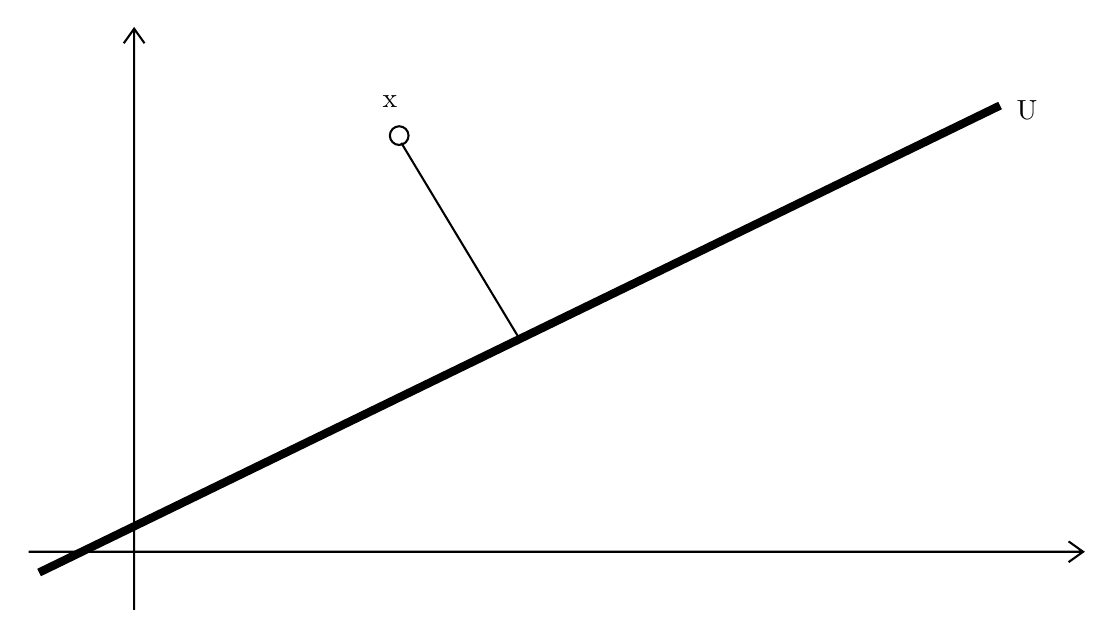
\begin{tikzpicture}[x=0.75pt,y=0.75pt,yscale=-1,xscale=1]
%uncomment if require: \path (0,300); %set diagram left start at 0, and has height of 300

%Shape: Axis 2D [id:dp7098119764904821] 
\draw  (50,256.93) -- (558,256.93)(100.8,4.93) -- (100.8,284.93) (551,251.93) -- (558,256.93) -- (551,261.93) (95.8,11.93) -- (100.8,4.93) -- (105.8,11.93)  ;
%Straight Lines [id:da9071558730776327] 
\draw [line width=3]    (55,266.93) -- (518,41.93) ;


%Straight Lines [id:da7398348018165936] 
\draw    (210,68.93) ;


%Shape: Circle [id:dp7764692603132283] 
\draw   (224,56.43) .. controls (224,53.95) and (226.01,51.93) .. (228.5,51.93) .. controls (230.99,51.93) and (233,53.95) .. (233,56.43) .. controls (233,58.92) and (230.99,60.93) .. (228.5,60.93) .. controls (226.01,60.93) and (224,58.92) .. (224,56.43) -- cycle ;
%Straight Lines [id:da721943207149605] 
\draw    (229.5,59.93) -- (286.5,154.43) ;



% Text Node
\draw (531,43.93) node  [align=left] {U};
% Text Node
\draw (224,39.93) node  [align=left] {x};


\end{tikzpicture}

		\caption{Skizze zur Bestapproximation}
		\label{Abb:Bestapproximation}
	\end{center}
\end{figure}

\begin{proof}
	\betone{Zeige \ref{item:satz2.10(1)}:}\\
	Sei $u\in U$ beliebig.
	Dann folgt aus der Definition der Projektion:
	\begin{align*}
		x=P_U(x)+v\qquad\exists v\in U^\perp\\
		\implies\norm{x-u}^2=\norm[\Big]{\big(\underbrace{P_U(x)-u}_{\in U}\big) +v}^2
		\overset{\ref{satz2.1}\ref{item:satz2.1(1)}}{=}
		\underbrace{\norm{P_U(x)-u}^2}_{\geq0}+\norm{v}^2
		\geq\norm{v}^2=\norm{x-P_U(x)}^2
	\end{align*}
	Und Gleichheit gilt genau dann, wenn $u=P_U(x)$.\nl
	\betone{Zeige \ref{item:satz2.10(2)}:}
	%TODO
	\betone{Zeige \ref{item:satz2.10(3)}:}
\end{proof}



